\documentclass[tikz,border=10pt]{standalone}
\usepackage{tikz}
\usetikzlibrary{positioning}

\begin{document}
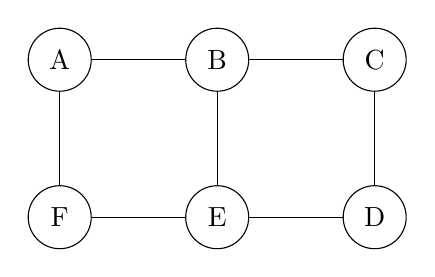
\begin{tikzpicture}[every node/.style={circle, draw, minimum size=8mm}]

% A graph of two squares stacked horizontally

\node (A) at (0,0) {A};
\node (B) at (2,0) {B};
\node (C) at (4,0) {C};
\node (D) at (4,-2) {D};
\node (E) at (2,-2) {E};
\node (F) at (0,-2) {F};

\draw (A) -- (B) -- (C) -- (D) -- (E) -- (F) -- (A);
\draw (B) -- (E);

\end{tikzpicture}
\end{document}